\documentclass[12pt]{article}
\usepackage{amssymb, amsmath, amsfonts, bm, graphicx, geometry}
\usepackage{tabularx, booktabs, float, enumitem, multicol, mathtools}
\geometry{margin=1in}


\title{}
\date{}
\author{}

\begin{document}
\begin{center}
{\LARGE ESC-201 Mechanics of Materials Notes\par}
\end{center}
The main idea of this course is to understand how mechanisms and designs perform under various loads and conditions. We will combine force loading from statics and dynamics with material properties to quantify the performance of a design and see how it fails.\\

{\centering\LARGE Basic Concepts\par}
\section*{Normal Stress}
\vspace{-1em}
\begin{minipage}[t]{0.6\textwidth} \vspace{0pt}
When load is applied normal to a cross-section such as the one below, we can find the normal stress applied by dividing the force by the area of the cross-section. This represents the \textit{average} normal stress, as the actual stress distribution is usually no uniform across the cross-section. It can be thought similarly to pressure, which both represents a load over an area.
\[\sigma_{\text{avg}} = \frac{P}{A}\]
\underline{Sign convention:} A positive stress corresponds to \textbf{tensile} loading while a negative stress corresponds to \textbf{compressive} loading.
\end{minipage}
\hfill
\begin{minipage}[t]{0.4\textwidth} \vspace{0pt}\centering
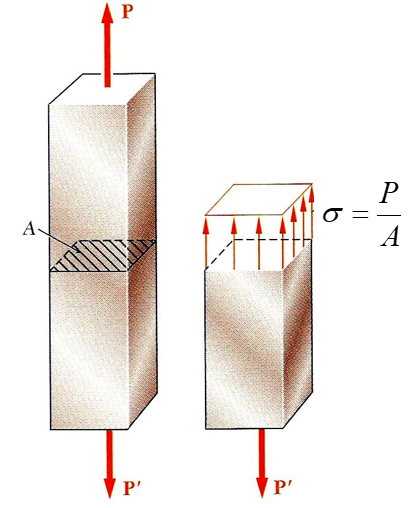
\includegraphics[width=\textwidth]{Normal Stress.png}
\end{minipage}
\section*{Shear Stress}
\vspace{-1em}
When load is applied parallel or along a cross-section, we can find the shear stress by dividing the force by the area of the cross-section. Similar to normal stress, this represents the \textit{average} shear stress, as the actual stress distribution is usually not uniform across the cross-section.
\[\tau_{\text{avg}} = \frac{P}{A}\]
\begin{center}
    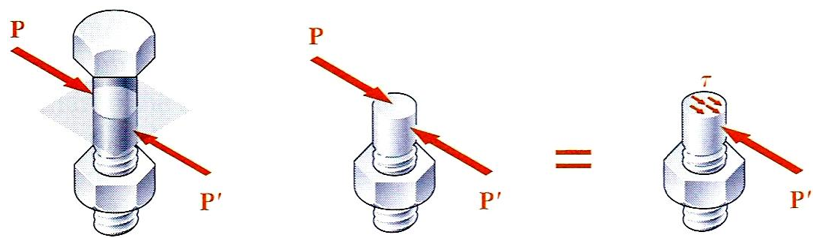
\includegraphics[width=0.8\textwidth]{Shear Stress.png}
\end{center}
\underline{Sign convention:} It follows the sign of the applied force. (ie. If the force is in the positive direction, the shear stress is positive.)\\\\
\underline{Note:} It is sometimes useful to think of stress as replacement for forces. For example, we can draw two different FBDs, one showing the forces and one showing the stresses.
\begin{center}
    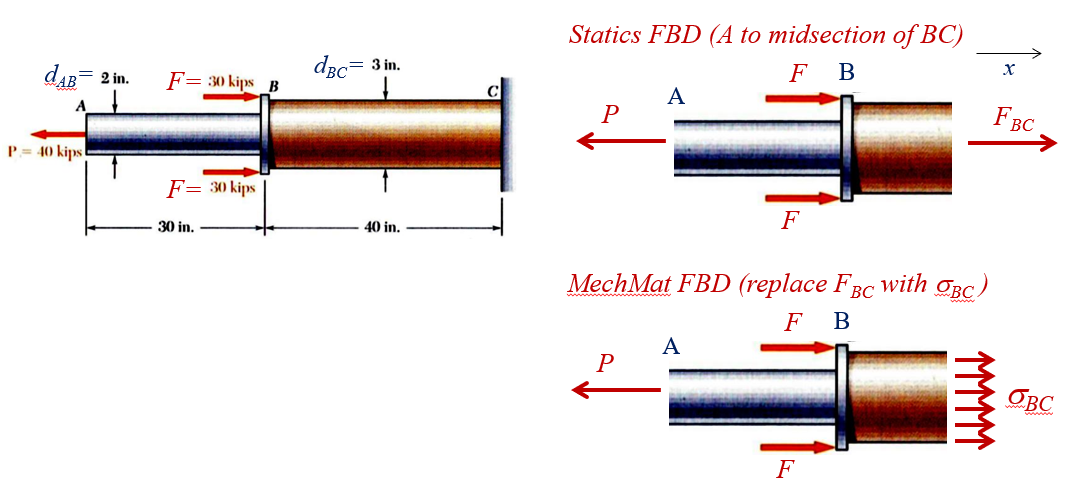
\includegraphics[width=1\textwidth]{Stress FBD.png}
\end{center}
\begin{minipage}[t]{0.4\textwidth} \vspace{0pt}
This way, it is clear to see what force corresponds to what stress and what area it acts on.\\\\

This is representative of our problem-solving approach. Starting from static force balances to solve for the forces, then using those forces to find the stresses, and finally using the stresses to find the strains and deformations.
\end{minipage}
\hfill
\begin{minipage}[t]{0.6\textwidth} \vspace{0pt}\centering
    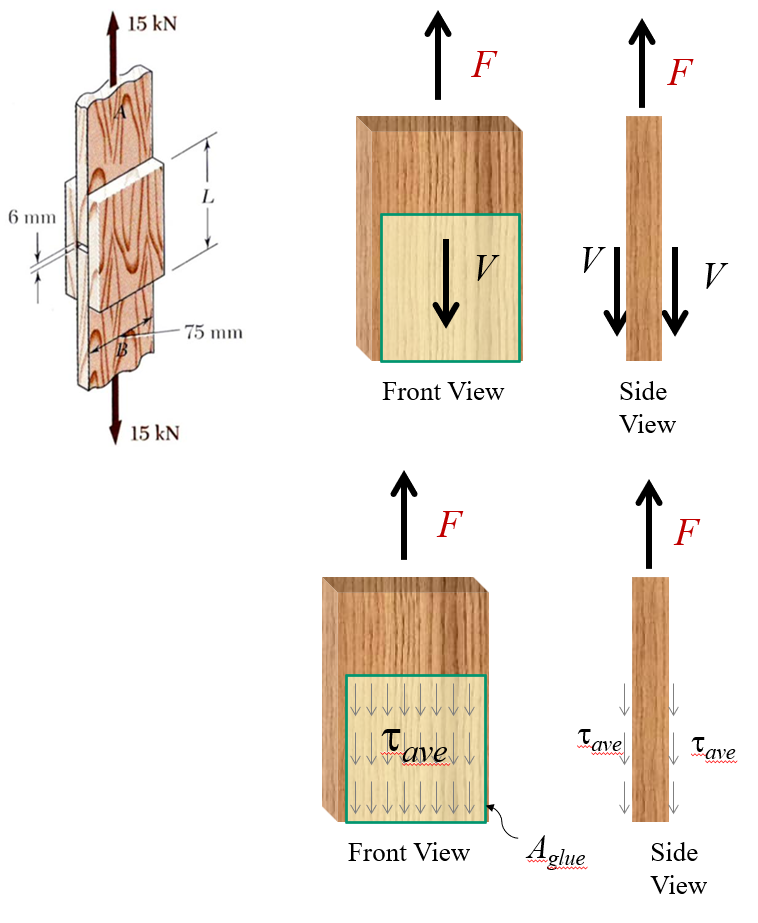
\includegraphics[width=\textwidth]{Stress FBD 1.png}
\end{minipage}
\section*{General Stress}
\vspace{-1em}
\begin{minipage}[t]{0.6\textwidth} \vspace{0pt}
When either the load is applied at an angle or the cross-section is not perpendicular to the load, we can always decompose the load into a normal and shear component. Then we can define the normal and shear stresses as before. 
\[\sigma = \frac{F}{A_{\theta}}=\frac{Pcos\theta}{A_{0}/cos\theta} = \frac{Pcos^2\theta}{A_0}\]
\[\tau = \frac{V}{A_{\theta}}=\frac{Psin\theta}{A_{0}/cos\theta} = \frac{Psin\theta cos\theta}{A_0}\]
Where $A_0$ is the area of the cross-section perpendicular to the load/axis and $A_{\theta}$ is the area of the cross-section at an angle $\theta$ to the load/axis.\\\\
\end{minipage}
\hfill
\begin{minipage}[t]{0.4\textwidth} \vspace{0pt}\centering
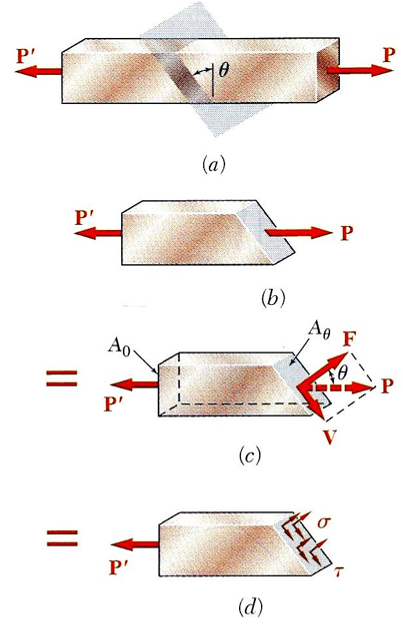
\includegraphics[width=\textwidth]{General Stress.png}
\end{minipage}
\section*{Pinned Joints}
\vspace{-1em}
When considering a pinned joint and how it fails, there are several ways. Mainly, it depends on whether the load is tensile or compressive. For both cases, the average normal stress at the midsection matters, but it's not usually where failure \textit{first} occurs, or in other words, it's not a critical region (it is usually where stress is max). The following are the critical regions unique to the type of loading:
\begin{itemize}
    \item \textbf{Member in Tension}\\
\begin{minipage}[t]{0.6\textwidth} \vspace{0pt}
Under tension, failure can occur by the member splitting at the shoulders around the pin where the cross-sectional area is smallest.
\[\sigma_{\text{avg}_\text{max}} = \frac{F_T}{A_{\text{min}}}\quad\text{(max average normal stress)}\]
Where $A_{\text{min}}$ is the minimum cross-sectional area of the member, which is usually defined by $(w-d)t$ where $w$ is the width of the member, $d$ is the diameter of the pin, and $t$ is the thickness of the member.
\end{minipage}
\hfill
\begin{minipage}[t]{0.4\textwidth} \vspace{0pt}\centering
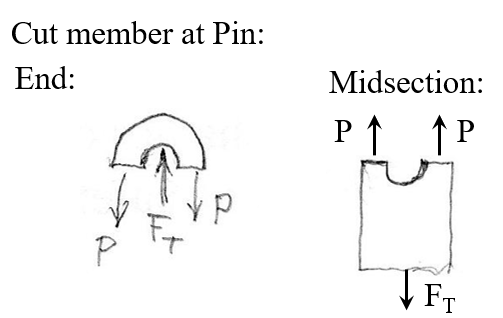
\includegraphics[width=\textwidth]{Tension-Stress.png}
\end{minipage}\newpage
\item \textbf{Member in Compression}\\
\begin{minipage}[t]{0.6\textwidth} \vspace{0pt}
Under compression, the pin squishes into the member and effectively becomes a solid piece. Thus, the risk isn't at the shoulders but rather at the midsection where it could buckle. Note that there is ZERO stress at the upper region around the hole since there is no load there.
\[\sigma_{\text{avg}} = \frac{F_C}{A_{\text{cross-section}}}\quad\text{(the usual average normal stress)}\]
\end{minipage}
\hfill
\begin{minipage}[t]{0.4\textwidth} \vspace{0pt}\centering
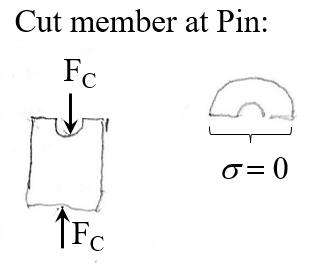
\includegraphics[width=\textwidth]{Compression-Stress.png}
\end{minipage}
\end{itemize}
For both cases, we need to also consider the shear stress on the pin and also the bearing stress on the member.\\\\
\textbf{Shear Stress at Pin}\\
\begin{minipage}[t]{0.6\textwidth} \vspace{0pt}
The first place failure can occur is that the pin shears. In this case, the pin is in \textit{single shear}. This is the same for both tension and compression.
\[\tau_{\text{avg}} = \frac{F_T}{A_{\text{pin}}}\]
Where $A_{\text{pin}}$ is the cross-sectional area of the pin.
\end{minipage}
\hfill
\begin{minipage}[t]{0.4\textwidth} \vspace{0pt}\centering
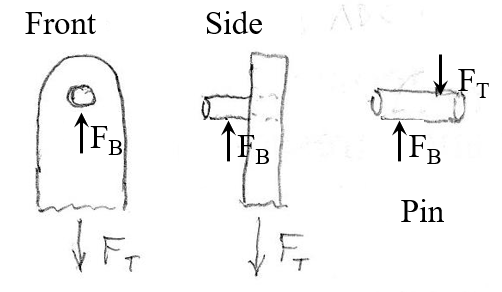
\includegraphics[width=\textwidth]{Tension-Shear.png}
\end{minipage}\\\\
\textbf{Bearing Stress}\\
\begin{minipage}[t]{0.6\textwidth} \vspace{0pt}
Another place failure can occur is that the hole the pin rests upon physically deforms and causes failure. This is called bearing stress, and it is always a compressive stress (the pin pushes into the hole). \\\\
It is also an average stress, but it uses the projected area of the bolt onto the hole:
\[\sigma_{\text{avg}} = \frac{P}{A_{\text{projected}}} = \frac{P}{td}\]
\underline{Sign convention:} Like mentioned before, this is always a compressive stress, so we report it as a positive value.
\end{minipage}
\hfill
\begin{minipage}[t]{0.4\textwidth} \vspace{0pt}\centering
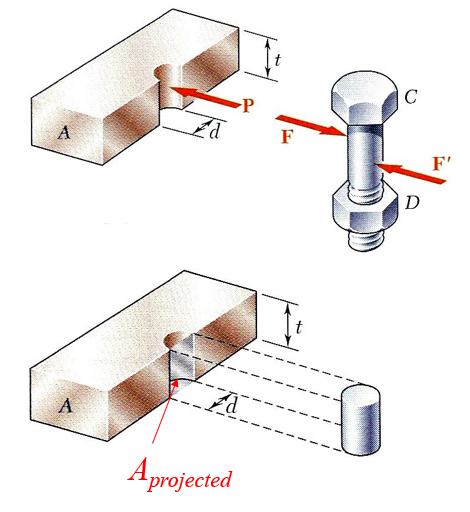
\includegraphics[width=\textwidth]{Bearing Stress.png}
\end{minipage}
\newpage
{\centering\LARGE Factor of Safety and Stresses\par}
\section*{Factor of Safety}
\vspace{-1em}
We use the factory of safety to compensate for using uniform stress assumptions and other variability. It is defined as 
\[\text{FS} = \frac{\text{Ultimate Load}}{\text{Allowable Load}}\]
Where the ultimate load is the max load at failure and the allowable load is the max design load. If failure is due to stress exceeding the ultimate strength, then
\[\text{FS} = \frac{\sigma_{\text{ult}}}{\sigma_{\text{allowable}}}\]
Where $\sigma_{\text{ult}}$ is the ultimate strength of the material and $\sigma_{\text{allowable}}$ is the allowable stress.
\section*{Shear in Pin or Bolt}
\vspace{-1em}
We've already mentioned single shear as a mode of failure for pinned joints, but here it is again:\\\\
\textbf{Single Shear}\\
Single shear means that there is one member per side of the pin, such that the shear load is \textit{equal} to the member/applied load. 
\[\tau_{\text{avg}} = \frac{\text{load}}{\text{pin XC area}}\]
\begin{center}
    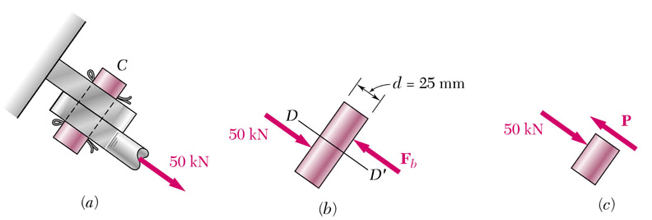
\includegraphics[width=0.8\textwidth]{Single Shear.png}
\end{center}
\textbf{Double Shear}\\
Double shear means shear is carried on both sides of incoming member (clevis joint) such that the load is split between two sides of clevis.
\[\tau_{\text{avg}} = \frac{\text{load}/2}{\text{pin XC area}}\]
\begin{center}
    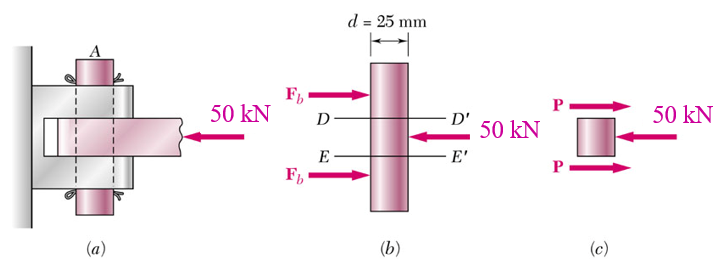
\includegraphics[width=0.8\textwidth]{Double Shear.png}
\end{center}
\begin{center}
    {\LARGE Axial Loading and Deformation\par}
\end{center}
This is going to be a long section, we finally introduce strain and deformation, allowing us to find things such as thermal stress, and solve for statically indeterminate problems.
\section*{Axial Strain}
\vspace{-1em}
\begin{minipage}[t]{0.6\textwidth} \vspace{0pt}
If deflection $\delta$ is defined as the change in length of a member (usually by some load), then we can define the axial strain as the amount of deflection per unit length. It is a dimensionless quantity.
\[\epsilon = \frac{\delta}{L}\quad\text{(uniform strain)}\]
For a general member, we can define the limit
\[\epsilon = \lim_{\delta\to 0} \frac{\Delta\delta}{\Delta L}=\frac{d\delta}{dL}\quad\text{(local strain)}\]
\end{minipage}
\hfill
\begin{minipage}[t]{0.4\textwidth} \vspace{0pt}\centering
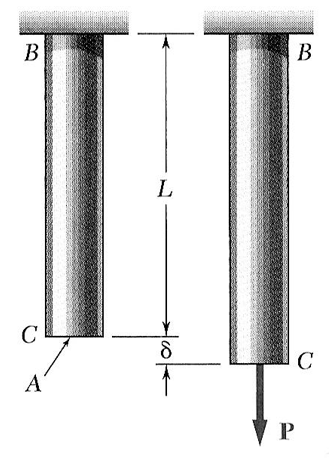
\includegraphics[width=\textwidth]{Axial Strain.png}
\end{minipage}
\vspace{-4em}
\section*{Axial Deflection}
In the elastic region below the yield stress, we can use Hooke's Law to relate the axial stress to the axial strain using Young's Modulus $E$.
\[\sigma = E\epsilon\] 
Thus, we can define the \textbf{axial deflection} as
\[\boxed{\delta = \frac{PL}{EA}}\]
and \textbf{stiffness} of the member as
\[\boxed{k = \frac{P}{\delta}=\frac{EA}{L}}\]
Note that $P$ is an \textit{internal} reaction force, not the applied load, so we must first solve for the internal forces using static force balances.
\begin{center}
    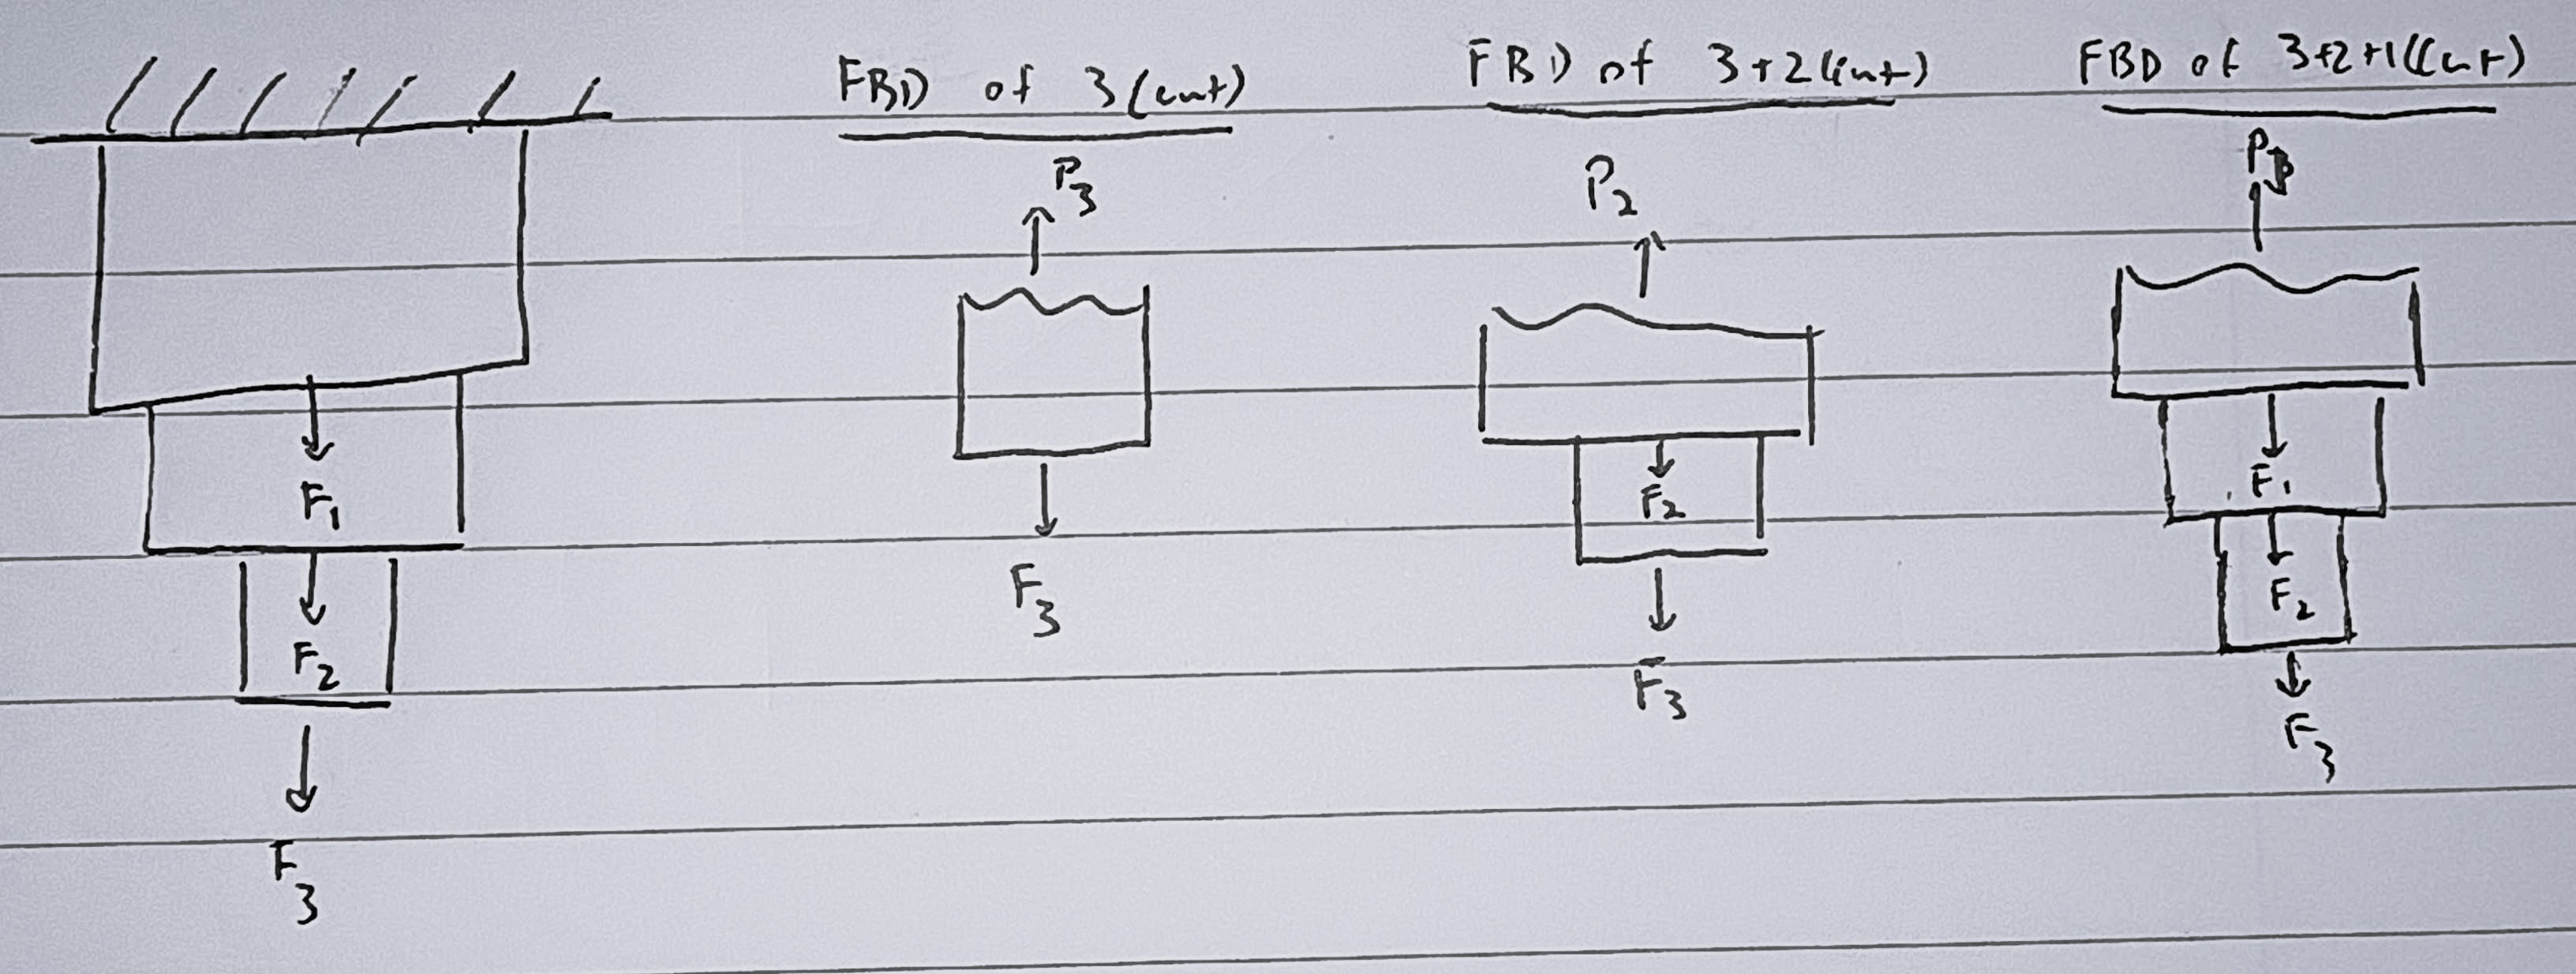
\includegraphics[width=0.8\textwidth]{Deflection FBD.jpg}
\end{center}
Thus, we can generalize for non-uniform members by integrating over the length of the member:
\[\delta = \sum\frac{P_i L_i}{E_i A_i} =\int_0^L \frac{P}{EA} dx\]
\section*{Statically Indeterminate Problems}
The nice thing about having a deflection formula is that we can now apply constraints on the deflection to solve for unknown forces. A useful analogy here is to think of the members as springs. In some cases, the members are in series where the total length is constant ($\delta_1 + \delta_2 = 0$), and in some cases, the members are in parallel where the deflection is constant ($\delta_1 = \delta_2$). We can use these constraints to solve for unknown forces and then find the stresses and strains as usual.
%Next up: prestressed concrete, thermal stress, poisson's ratio, and stress concentration factors.

\end{document}